% A LaTeX template for EXECUTIVE SUMMARY of the MSc Thesis submissions to 
% Politecnico di Milano (PoliMi) - School of Industrial and Information Engineering
%
% S. Bonetti, A. Gruttadauria, G. Mescolini, A. Zingaro
% e-mail: template-tesi-ingind@polimi.it
%
% Last Revision: October 2021
%
% Copyright 2021 Politecnico di Milano, Italy. NC-BY

\documentclass[11pt,a4paper,twocolumn]{article}

%------------------------------------------------------------------------------
%	REQUIRED PACKAGES AND  CONFIGURATIONS
%------------------------------------------------------------------------------
% PACKAGES FOR TITLES
\usepackage{titlesec}
\usepackage{color}

% PACKAGES FOR LANGUAGE AND FONT
\usepackage[utf8]{inputenc}
\usepackage[english]{babel}
\usepackage[T1]{fontenc} % Font encoding

% PACKAGES FOR IMAGES
\usepackage{graphicx}
\usepackage{tikz} % A package for high-quality hand-made figures.
\usetikzlibrary{}
\graphicspath{{./Images/}} % Directory of the images
\usepackage{eso-pic} % For the background picture on the title page
\usepackage{subfig} % Numbered and caption subfigures using \subfloat
\usepackage{caption} % Coloured captions
\usepackage{transparent}

% STANDARD MATH PACKAGES
\usepackage{amsmath}
\usepackage{amsthm}
\usepackage{bm}
\usepackage[overload]{empheq}  % For braced-style systems of equations

% PACKAGES FOR TABLES
\usepackage{tabularx}
\usepackage{longtable} % tables that can span several pages
\usepackage{colortbl}

% PACKAGES FOR ALGORITHMS (PSEUDO-CODE)
\usepackage{algorithm}
\usepackage{algorithmic}

% PACKAGES FOR REFERENCES & BIBLIOGRAPHY
\usepackage[colorlinks=true,linkcolor=black,anchorcolor=black,citecolor=black,filecolor=black,menucolor=black,runcolor=black,urlcolor=black]{hyperref} % Adds clickable links at references
\usepackage{cleveref}
\usepackage[authoryear, square, numbers, sort&compress]{natbib} % Square brackets, citing references with numbers, citations sorted by appearance in the text and compressed
\bibliographystyle{apalike} % You may use a different style adapted to your field

% PACKAGES FOR THE APPENDIX
\usepackage{appendix}

% PACKAGES FOR ITEMIZE & ENUMERATES 
\usepackage{enumitem}

% OTHER PACKAGES
\usepackage{amsthm,thmtools,xcolor} % Coloured "Theorem"
\usepackage{comment} % Comment part of code
\usepackage{fancyhdr} % Fancy headers and footers
\usepackage{lipsum} % Insert dummy text
\usepackage{tcolorbox} % Create coloured boxes (e.g. the one for the key-words)
\usepackage{stfloats} % Correct position of the tables

%-------------------------------------------------------------------------
%	NEW COMMANDS DEFINED
%-------------------------------------------------------------------------
% EXAMPLES OF NEW COMMANDS -> here you see how to define new commands
\newcommand{\bea}{\begin{eqnarray}} % Shortcut for equation arrays
\newcommand{\eea}{\end{eqnarray}}
\newcommand{\e}[1]{\times 10^{#1}}  % Powers of 10 notation
\newcommand{\mathbbm}[1]{\text{\usefont{U}{bbm}{m}{n}#1}} % From mathbbm.sty
\newcommand{\pdev}[2]{\frac{\partial#1}{\partial#2}}
% NB: you can also override some existing commands with the keyword \renewcommand

%----------------------------------------------------------------------------
%	ADD YOUR PACKAGES (be careful of package interaction)
%----------------------------------------------------------------------------
\usepackage{adjustbox}
\usepackage{enumitem}

%----------------------------------------------------------------------------
%	ADD YOUR DEFINITIONS AND COMMANDS (be careful of existing commands)
%----------------------------------------------------------------------------


% Do not change Configuration_files/config.tex file unless you really know what you are doing. 
% This file ends the configuration procedures (e.g. customizing commands, definition of new commands)
% Set the geometric layout of the document
\usepackage{geometry}
\geometry{
  top=3cm,
  left = 2.0cm,
  right = 2.0cm,
  bottom=2cm,
  headheight= 2cm,
  headsep= 0cm,
}
\raggedbottom 

% Create color bluePoli (-> manuale grafica coordinata:  https://www.polimi.it/fileadmin/user_upload/il_Politecnico/grafica-coordinata/2015_05_11_46xy_manuale_grafica_coordinata.pdf)
\definecolor{bluePoli}{cmyk}{0.4,0.1,0,0.4}

% Custom theorem environments
\declaretheoremstyle[
  headfont=\color{bluePoli}\normalfont\bfseries,
  bodyfont=\color{black}\normalfont\itshape,
]{colored}

\captionsetup[figure]{labelfont={color=bluePoli}} % Set colour of the captions
\captionsetup[table]{labelfont={color=bluePoli}} % Set colour of the captions
\captionsetup[algorithm]{labelfont={color=bluePoli}} % Set colour of the captions

\theoremstyle{colored}
\newtheorem{theorem}{Theorem}[section]
\newtheorem{proposition}{Proposition}[section]

% Enhances the features of the standard "table" and "tabular" environments.
\newcommand\T{\rule{0pt}{2.6ex}}
\newcommand\B{\rule[-1.2ex]{0pt}{0pt}}

% Algorithm description
\newcounter{algsubstate}
\renewcommand{\thealgsubstate}{\alph{algsubstate}}
\newenvironment{algsubstates}{
    \setcounter{algsubstate}{0}%
    \renewcommand{\STATE}{%
    \stepcounter{algsubstate}%
    \Statex {\small\thealgsubstate:}\space}
    }{}
    
% Custom theorem environment
\newcolumntype{L}[1]{>{\raggedright\let\newline\\\arraybackslash\hspace{0pt}}m{#1}}
\newcolumntype{C}[1]{>{\centering\let\newline\\\arraybackslash\hspace{0pt}}m{#1}}
\newcolumntype{R}[1]{>{\raggedleft\let\newline\\\arraybackslash\hspace{0pt}}m{#1}}

% Custom itemize environment
\setlist[itemize,1]{label=$\bullet$}
\setlist[itemize,2]{label=$\circ$}
\setlist[itemize,3]{label=$-$}
\setlist{nosep}

% Set separation of columns 
\setlength{\columnsep}{30pt}

% Create command for background pic
\newcommand\BackgroundPic{% Adding background picture
	\put(230,358){
		\parbox[b][\paperheight]{\paperwidth}{%
			\vfill
			\centering
			\transparent{0.4}
			
\includegraphics[width=0.5\paperwidth]{raggiera_polimi.eps}%
			\vfill
}}}

% Set indentation
\setlength\parindent{0pt}

% Custom title commands
\titleformat{\section}
{\color{bluePoli}\normalfont\Large\bfseries}
{\color{bluePoli}\thesection.}{1em}{}
\titlespacing*{\section}
{0pt}{2ex}{1ex}

\titleformat{\subsection}
{\color{bluePoli}\normalfont\large\bfseries}
{\color{bluePoli}\thesubsection.}{1em}{}
\titlespacing*{\subsection}
{0pt}{2ex}{1ex}

% Custom headers and footers
\pagestyle{fancy}
\fancyhf{}
      
\fancyfoot{}
\fancyfoot[C]{\thepage} % page
\renewcommand{\headrulewidth}{0mm} % headrule width
\renewcommand{\footrulewidth}{0mm} % footrule width

\makeatletter
\patchcmd{\headrule}{\hrule}{\color{black}\hrule}{}{} % headrule
\patchcmd{\footrule}{\hrule}{\color{black}\hrule}{}{} % footrule
\makeatother

% -> Create the header
\chead[C]{
\centering
\begin{tcolorbox}[arc=0pt, boxrule=0pt, colback=bluePoli!60, width=\textwidth, colupper=white]
    \textbf{Executive summary} \hfill \textbf{\author}  
\end{tcolorbox}
}

% Insert here the info that will be displayed into your Title page 
% -> title of your work
\renewcommand{\title}{Three-dimensional bin packing with vertical support}
% -> author name and surname
\renewcommand{\author}{Jacopo Libè}
% -> MSc course
\newcommand{\course}{Computer Science and Engineering - Ingegneria Informatica}
% -> advisor name and surname
\newcommand{\advisor}{Prof. Ola Jabali}
% IF AND ONLY IF you need to modify the co-supervisors you also have to modify the file Configuration_files/title_page.tex (ONLY where it is marked)
\newcommand{\firstcoadvisor}{Davide Croci} % insert if any otherwise comment
%\newcommand{\secondcoadvisor}{Name Surname} % insert if any otherwise comment
% -> academic year
\newcommand{\YEAR}{2021-2022}

%-------------------------------------------------------------------------
%	BEGIN OF YOUR DOCUMENT
%-------------------------------------------------------------------------
\begin{document}

%-----------------------------------------------------------------------------
% TITLE PAGE
%-----------------------------------------------------------------------------
% Do not change Configuration_files/TitlePage.tex (Modify it IF AND ONLY IF you need to add or delete the Co-advisors)
% This file creates the Title Page of the document
% DO NOT REMOVE SPACES BETWEEN LINES!

\twocolumn[{\begin{@twocolumnfalse}

    \AddToShipoutPicture*{\BackgroundPic}
    
    \hspace{-0.6cm}
\includegraphics[width=0.6\textwidth]{logo_polimi_ing_indinf.eps}
    
    \vspace{-1mm}
    \fontsize{0.3cm}{0.5cm}\selectfont \bfseries \textsc{\color{bluePoli} Executive Summary of the Thesis}\\
    
    \vspace{-0.2cm}
    \Large{\textbf{\color{bluePoli}{\title}}}\\
    
    \vspace{-0.2cm}
    \fontsize{0.3cm}{0.5cm}\selectfont \bfseries \textsc{\color{bluePoli} Laurea Magistrale in \course}\\
    
    \vspace{-0.2cm}
    \fontsize{0.3cm}{0.5cm} \selectfont \bfseries Author: \textsc{\textbf{\author}}\\
    
    \vspace{-0.4cm}
    \fontsize{0.3cm}{0.5cm}\selectfont \bfseries Advisor: \textsc{\textbf{\advisor}}\\
    
    % if only ONE co-advisor is present:
    \vspace{-0.4cm}
    \fontsize{0.3cm}{0.5cm}\selectfont \bfseries Co-advisor: \textsc{\textbf{\firstcoadvisor}}\\
    % if more than one co-advisors are present:
    %\vspace{-0.4cm}
    %\fontsize{0.3cm}{0.5cm}\selectfont \bfseries Co-advisors: \textsc{\textbf{\firstcoadvisor}}\textsc{\textbf{\secondcoadvisor}}\\
    
    \vspace{-0.4cm}
    \fontsize{0.3cm}{0.5cm}\selectfont \bfseries Academic year: \textsc{\textbf{\YEAR}}
    
    \small \normalfont
    
    \vspace{11pt}
    
    \centerline{\rule{1.0\textwidth}{0.4pt}}
    
    \vspace{15pt}
    \end{@twocolumnfalse}}]
    
    \thispagestyle{plain} % In order to not show the header in the first page

%%%%%%%%%%%%%%%%%%%%%%%%%%%%%%
%%     THESIS MAIN TEXT     %%
%%%%%%%%%%%%%%%%%%%%%%%%%%%%%%



%% \section{Guidelines}
%% \label{sec:guidelines}
%% 
%% The Executive Summary is a critical overview of your thesis
%% with a focus on the main achievements that have emerged from your research.
%% 
%% The Executive Summary should be organized in sections/paragraphs
%% in order to better highlight the major points of your work.
%% The length should range from four to six pages depending on the length of the thesis manuscript.
%% Keep the Executive Summary concise enough to be effective but long enough to allow it to be complete.
%% It should be written after completing the thesis manuscript as a stand-alone independent document
%% of sufficient clarity and detail to ensure that the reader can figure out the overall objectives,
%% the methodology employed and the results/impact of your research.
%% 
%% In writing the Executive Summary, keep in mind that it is not an abstract, it is not a preface,
%% and it is not a random collection of highlights.
%% With a few exceptions, do not simply cut and paste whole sections or paragraphs of the thesis manuscript
%% into a disorganized and cluttered Executive Summary.
%% You should reorganize information to be informative as well as concise.
%% 
%% The Executive Summary could contain a few important equations related to your work.
%% It could also include the most relevant figures and tables taken or elaborated from the thesis manuscript.
%% 
%% You should also include in the Executive Summary the very essential bibliography of your study.
%% The number of selected references should range from three to five depending on the type of work.
%% 
%% The Executive Summary should contain a final section reporting the main conclusions drawn from your research.

%-----------------------------------------------------------------------------
% INTRODUCTION
%-----------------------------------------------------------------------------
\section{Introduction}
\label{sec:introduction}

Recent progress in the digitalization of industrial processes led to a rise in studies on the Three-Dimensional Bin Packing Problem (3D-BPP).
The problem consists in packing a set of items in the minimum number of bins without any overlap.
When considering real-world settings, the addition of new practical constraints is required.
Previous studies in other fields related to container loading and pallet loading have shown that static stability of the bins is a crucial aspect to consider (\cite{BORTFELDT20131}).
In this thesis, we address a version of the bin packing problem stemming from a real case study of mixed-case palletization: the Three-Dimensional Bin Packing Problem with Vertical Support (3D-BPPVS).
We extend the standard formulation of the bin packing problem by ensuring that all items that are packed inside a bin will not fall, and we refer to this property as the vertical support.
Vertical stability is usually ensured between horizontal or vertical slices of items as a constraint on the minimum amount of area which rests on other items (e.g., \cite{GZARA20201062,paquay2016mixed}).
Each item can also be rotated along its vertical axis by 90 degrees.

Our research stems from the case study of a logistics company in northern Italy.
The company manages large warehouses where automated lines bring boxes to different packing stations, and then they are loaded onto pallets of standard size.
Since the company is dealing directly with customers' orders, boxes have very different sizes and are usually packed in smaller quantities.
Moreover, the assortment of items to pack is strongly heterogeneous which makes the use of layered approaches have sub-optimal results.
During the palletization, levels of already packed items are wrapped to ensure better overall stability of the pallet.
This wrapping procedure requires that the amount of unused space between items is minimal.
The company measures this property with a metric called cage ratio.
Cage ratio is the ratio between the volume of the packed items inside a bin and the volume of the cuboid which surrounds them, the cage.
The cage has the same base as the bin and height equal to the highest packed item inside the bin.
Current commercial solutions employed by the company have solutions with around $60\%$ cage ratio, and a target of $70\%$ was set as a benchmark for our work.
A visual representation of the cage ratio is shown in \cref{fig:cage_ratio}.

\begin{figure}[h]
    \resizebox{\columnwidth}{!}{%
    

\tikzset{every picture/.style={line width=0.75pt}} %set default line width to 0.75pt        

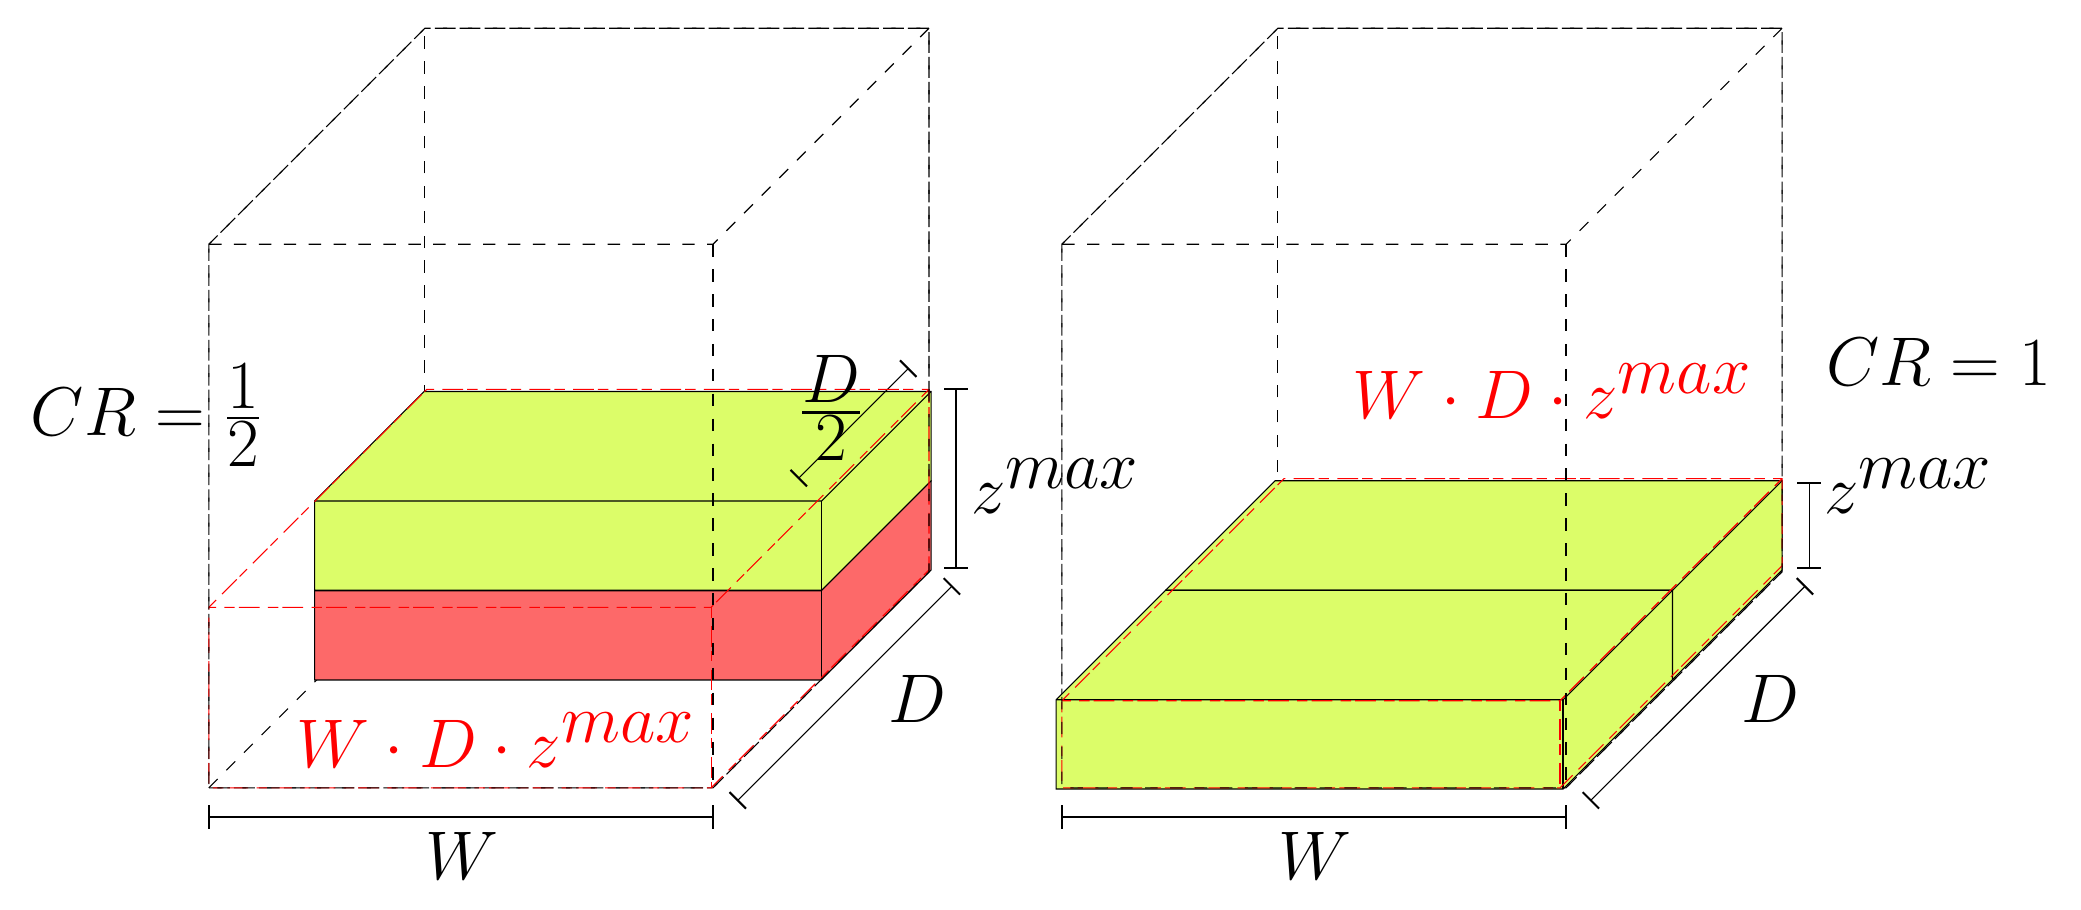
\begin{tikzpicture}[x=0.75pt,y=0.75pt,yscale=-1,xscale=1,font={\fontsize{50pt}{12}\selectfont}]
%uncomment if require: \path (0,479); %set diagram left start at 0, and has height of 479

%Shape: Cube [id:dp9446615397697055] 
\draw  [dash pattern={on 4.5pt off 4.5pt}] (917,301.9) -- (812.9,406) -- (570,406) -- (570,144.1) -- (674.1,40) -- (917,40) -- cycle ; \draw  [dash pattern={on 4.5pt off 4.5pt}] (570,406) -- (674.1,301.9) -- (917,301.9) ; \draw  [dash pattern={on 4.5pt off 4.5pt}] (674.1,301.9) -- (674.1,40) ;
%Shape: Cube [id:dp9924623151681093] 
\draw  [fill={rgb, 255:red, 220; green, 253; blue, 105 }  ,fill opacity=1 ] (620,310.78) -- (672.78,258) -- (917,258) -- (917,301) -- (864.22,353.78) -- (620,353.78) -- cycle ; \draw   (917,258) -- (864.22,310.78) -- (620,310.78) ; \draw   (864.22,310.78) -- (864.22,353.78) ;
%Shape: Cube [id:dp4356357707795666] 
\draw  [fill={rgb, 255:red, 220; green, 253; blue, 105 }  ,fill opacity=1 ] (567.22,363.56) -- (620,310.78) -- (864.22,310.78) -- (864.22,353.78) -- (811.44,406.56) -- (567.22,406.56) -- cycle ; \draw   (864.22,310.78) -- (811.44,363.56) -- (567.22,363.56) ; \draw   (811.44,363.56) -- (811.44,406.56) ;
%Shape: Cube [id:dp900981008021689] 
\draw  [dash pattern={on 4.5pt off 4.5pt}] (506,301.9) -- (401.9,406) -- (159,406) -- (159,144.1) -- (263.1,40) -- (506,40) -- cycle ; \draw  [dash pattern={on 4.5pt off 4.5pt}] (159,406) -- (263.1,301.9) -- (506,301.9) ; \draw  [dash pattern={on 4.5pt off 4.5pt}] (263.1,301.9) -- (263.1,40) ;
%Shape: Cube [id:dp9462720863667783] 
\draw  [fill={rgb, 255:red, 253; green, 105; blue, 105 }  ,fill opacity=1 ] (210,311) -- (263,258) -- (507,258) -- (507,301) -- (454,354) -- (210,354) -- cycle ; \draw   (507,258) -- (454,311) -- (210,311) ; \draw   (454,311) -- (454,354) ;
%Shape: Cube [id:dp20686523528460465] 
\draw  [fill={rgb, 255:red, 220; green, 253; blue, 105 }  ,fill opacity=1 ] (210,267.78) -- (262.78,215) -- (507,215) -- (507,258) -- (454.22,310.78) -- (210,310.78) -- cycle ; \draw   (507,215) -- (454.22,267.78) -- (210,267.78) ; \draw   (454.22,267.78) -- (454.22,310.78) ;
%Straight Lines [id:da9583369995131138] 
\draw    (496,204) -- (443.22,256.78) ;
\draw [shift={(443.22,256.78)}, rotate = 315] [color={rgb, 255:red, 0; green, 0; blue, 0 }  ][line width=0.75]    (0,5.59) -- (0,-5.59)   ;
\draw [shift={(496,204)}, rotate = 315] [color={rgb, 255:red, 0; green, 0; blue, 0 }  ][line width=0.75]    (0,5.59) -- (0,-5.59)   ;
%Straight Lines [id:da4480701288134522] 
\draw    (401.9,420) -- (159,420) ;
\draw [shift={(159,420)}, rotate = 360] [color={rgb, 255:red, 0; green, 0; blue, 0 }  ][line width=0.75]    (0,5.59) -- (0,-5.59)   ;
\draw [shift={(401.9,420)}, rotate = 360] [color={rgb, 255:red, 0; green, 0; blue, 0 }  ][line width=0.75]    (0,5.59) -- (0,-5.59)   ;
%Straight Lines [id:da9761873387202039] 
\draw    (517,308.9) -- (413.86,412) ;
\draw [shift={(413.86,412)}, rotate = 315.01] [color={rgb, 255:red, 0; green, 0; blue, 0 }  ][line width=0.75]    (0,5.59) -- (0,-5.59)   ;
\draw [shift={(517,308.9)}, rotate = 315.01] [color={rgb, 255:red, 0; green, 0; blue, 0 }  ][line width=0.75]    (0,5.59) -- (0,-5.59)   ;
%Straight Lines [id:da1211437330301477] 
\draw    (519,214) -- (519,299.86) ;
\draw [shift={(519,299.86)}, rotate = 270] [color={rgb, 255:red, 0; green, 0; blue, 0 }  ][line width=0.75]    (0,5.59) -- (0,-5.59)   ;
\draw [shift={(519,214)}, rotate = 270] [color={rgb, 255:red, 0; green, 0; blue, 0 }  ][line width=0.75]    (0,5.59) -- (0,-5.59)   ;
%Shape: Cube [id:dp6016430781165488] 
\draw  [color={rgb, 255:red, 255; green, 0; blue, 0 }  ,draw opacity=1 ][dash pattern={on 3.75pt off 3pt on 7.5pt off 1.5pt}] (159,319) -- (264,214) -- (506,214) -- (506,301) -- (401,406) -- (159,406) -- cycle ; \draw  [color={rgb, 255:red, 255; green, 0; blue, 0 }  ,draw opacity=1 ][dash pattern={on 3.75pt off 3pt on 7.5pt off 1.5pt}] (506,214) -- (401,319) -- (159,319) ; \draw  [color={rgb, 255:red, 255; green, 0; blue, 0 }  ,draw opacity=1 ][dash pattern={on 3.75pt off 3pt on 7.5pt off 1.5pt}] (401,319) -- (401,406) ;
%Shape: Cube [id:dp9858212525551202] 
\draw  [dash pattern={on 4.5pt off 4.5pt}] (159,144.1) -- (263.1,40) -- (506,40) -- (506,301.9) -- (401.9,406) -- (159,406) -- cycle ; \draw  [dash pattern={on 4.5pt off 4.5pt}] (506,40) -- (401.9,144.1) -- (159,144.1) ; \draw  [dash pattern={on 4.5pt off 4.5pt}] (401.9,144.1) -- (401.9,406) ;
%Straight Lines [id:da4537070040642701] 
\draw    (812.9,420) -- (570,420) ;
\draw [shift={(570,420)}, rotate = 360] [color={rgb, 255:red, 0; green, 0; blue, 0 }  ][line width=0.75]    (0,5.59) -- (0,-5.59)   ;
\draw [shift={(812.9,420)}, rotate = 360] [color={rgb, 255:red, 0; green, 0; blue, 0 }  ][line width=0.75]    (0,5.59) -- (0,-5.59)   ;
%Straight Lines [id:da13051427322471099] 
\draw    (928,308.9) -- (824.86,412) ;
\draw [shift={(824.86,412)}, rotate = 315.01] [color={rgb, 255:red, 0; green, 0; blue, 0 }  ][line width=0.75]    (0,5.59) -- (0,-5.59)   ;
\draw [shift={(928,308.9)}, rotate = 315.01] [color={rgb, 255:red, 0; green, 0; blue, 0 }  ][line width=0.75]    (0,5.59) -- (0,-5.59)   ;
%Straight Lines [id:da38828166025774113] 
\draw    (930,259) -- (930,299.86) ;
\draw [shift={(930,299.86)}, rotate = 270] [color={rgb, 255:red, 0; green, 0; blue, 0 }  ][line width=0.75]    (0,5.59) -- (0,-5.59)   ;
\draw [shift={(930,259)}, rotate = 270] [color={rgb, 255:red, 0; green, 0; blue, 0 }  ][line width=0.75]    (0,5.59) -- (0,-5.59)   ;
%Shape: Cube [id:dp33203292048167843] 
\draw  [color={rgb, 255:red, 255; green, 0; blue, 0 }  ,draw opacity=1 ][dash pattern={on 3.75pt off 3pt on 7.5pt off 1.5pt}] (570,364) -- (677,257) -- (917,257) -- (917,299) -- (810,406) -- (570,406) -- cycle ; \draw  [color={rgb, 255:red, 255; green, 0; blue, 0 }  ,draw opacity=1 ][dash pattern={on 3.75pt off 3pt on 7.5pt off 1.5pt}] (917,257) -- (810,364) -- (570,364) ; \draw  [color={rgb, 255:red, 255; green, 0; blue, 0 }  ,draw opacity=1 ][dash pattern={on 3.75pt off 3pt on 7.5pt off 1.5pt}] (810,364) -- (810,406) ;
%Shape: Cube [id:dp6959350788468752] 
\draw  [dash pattern={on 4.5pt off 4.5pt}] (570,144.1) -- (674.1,40) -- (917,40) -- (917,301.9) -- (812.9,406) -- (570,406) -- cycle ; \draw  [dash pattern={on 4.5pt off 4.5pt}] (917,40) -- (812.9,144.1) -- (570,144.1) ; \draw  [dash pattern={on 4.5pt off 4.5pt}] (812.9,144.1) -- (812.9,406) ;

% Text Node
\draw (442,196.4) node [anchor=north west][inner sep=0.75pt]    {$\frac{D}{2}$};
% Text Node
\draw (262,426.4) node [anchor=north west][inner sep=0.75pt]    {$W$};
% Text Node
\draw (485,350.4) node [anchor=north west][inner sep=0.75pt]    {$D$};
% Text Node
\draw (72,200.4) node [anchor=north west][inner sep=0.75pt]    {$CR=\frac{1}{2}$};
% Text Node
\draw (525,246.4) node [anchor=north west][inner sep=0.75pt]    {$z^{max}$};
% Text Node
\draw (200,368.4) node [anchor=north west][inner sep=0.75pt]  [color={rgb, 255:red, 255; green, 0; blue, 0 }  ,opacity=1 ]  {$W\cdot D\cdot z^{max}$};
% Text Node
\draw (673,426.4) node [anchor=north west][inner sep=0.75pt]    {$W$};
% Text Node
\draw (896,350.4) node [anchor=north west][inner sep=0.75pt]    {$D$};
% Text Node
\draw (937,188.4) node [anchor=north west][inner sep=0.75pt]    {$CR=1$};
% Text Node
\draw (936,246.4) node [anchor=north west][inner sep=0.75pt]    {$z^{max}$};
% Text Node
\draw (709,200.4) node [anchor=north west][inner sep=0.75pt]  [color={rgb, 255:red, 255; green, 0; blue, 0 }  ,opacity=1 ]  {$W\cdot D\cdot z^{max}$};


\end{tikzpicture}

    }
    \caption{Cage ratio of two different bin configurations}
    \label{fig:cage_ratio}
\end{figure}

\section{Literature Review}
The 3D-BPP is the generalization of the one-dimensional bin packing problem which is NP-Hard (\cite{martello2000three}).
Exact methods can only solve small instances of the problem which means that most solutions proposed in the literature are heuristics.
Heuristics for the 3D-BPP are designed to solve the standard problem and don't take into account practical constraints.
\cite{martello2000three} provided a set of benchmark instances for 3D-BPP heuristics, and an exact method based on a two-level branch-and-bound algorithm.
Their method used a staircase placement strategy, where a series of corner points were identified as possible placement points to evaluate.
The method was later extended in \cite{crainic2008extreme} to find new niches previously ignored by the introduction of Extreme Points.
\cite{gonccalves2013biased} introduced a biased random-key genetic algorithm (BRKGA) which is one of the best performing heuristics on the benchmark instances of \cite{martello2000three}.
The algorithm was later modified with variable neighborhood descent variation presented in \cite{zudio2018brkga} which improved the number of generations needed to find high-quality results.

The concept of vertical support received most of its contribution from the literature of Container Loading Problems (CLP) and Pallet Loading Problems (PLP).
As noted in \cite{BORTFELDT20131}, static stability is usually implicitly enforced as a consequence of load compactness, or explicitly guaranteed by using filler material in a post-processing step.
Most heuristics for CLPS and PLPs try to build dense layers composed of similar items that they stack, reducing the problem to a one-dimensional bin packing problem.
Layers are filtered based on the fill-rate and when they are below a certain threshold they are discarded (e.g., \cite{elhedhli2019three, Alonso2020}).
This means that when no new layer can be built, new bins are opened, simpler placement methods are used to pack the remaining items or filler material is used to complete the layers.
Other more recent methods in the PLPs literature ensure support explicitly as a post-processing step when spacing layers relative to eachother (e.g., \cite{GZARA20201062}).

Our solution to the problem fills the gap in the research by finding solutions to the 3D-BPPVS without explicitly building layers, and without the use of filler material.

\section{Proposed Solution}

Based on other publications from the literature and our case study partner's insights we define the property of vertical support.
Given a support area threshold $\alpha_s$ and a maximum vertical gap below which an item can be considered as effectively supporting another one $\beta_s$. We define an item as supported if one of the following conditions holds
\begin{enumerate}[label={\textbf{Condition \arabic*}.},ref={\arabic*},leftmargin=*]
    \item the sum of the overlap area over the XY-plane with every other item on which it is resting is greater than $\alpha_s$ times its base area. (area support) \label{support:area_support}
    \item the number of its corners resting on another item is greater or equal to 3, and condition \ref{support:area_support} holds with a threshold $\alpha^\prime_s$ where $\alpha^\prime_s < \alpha_s$. (vertex support) \label{support:vertex_support}
\end{enumerate}
A visual representation of the conditions \ref{support:area_support} and \ref{support:vertex_support} of support is illustrated in \cref{fig:support}.

\begin{figure}[h]
    \resizebox{\columnwidth}{!}{%
    

\tikzset{every picture/.style={line width=0.75pt}} %set default line width to 0.75pt        

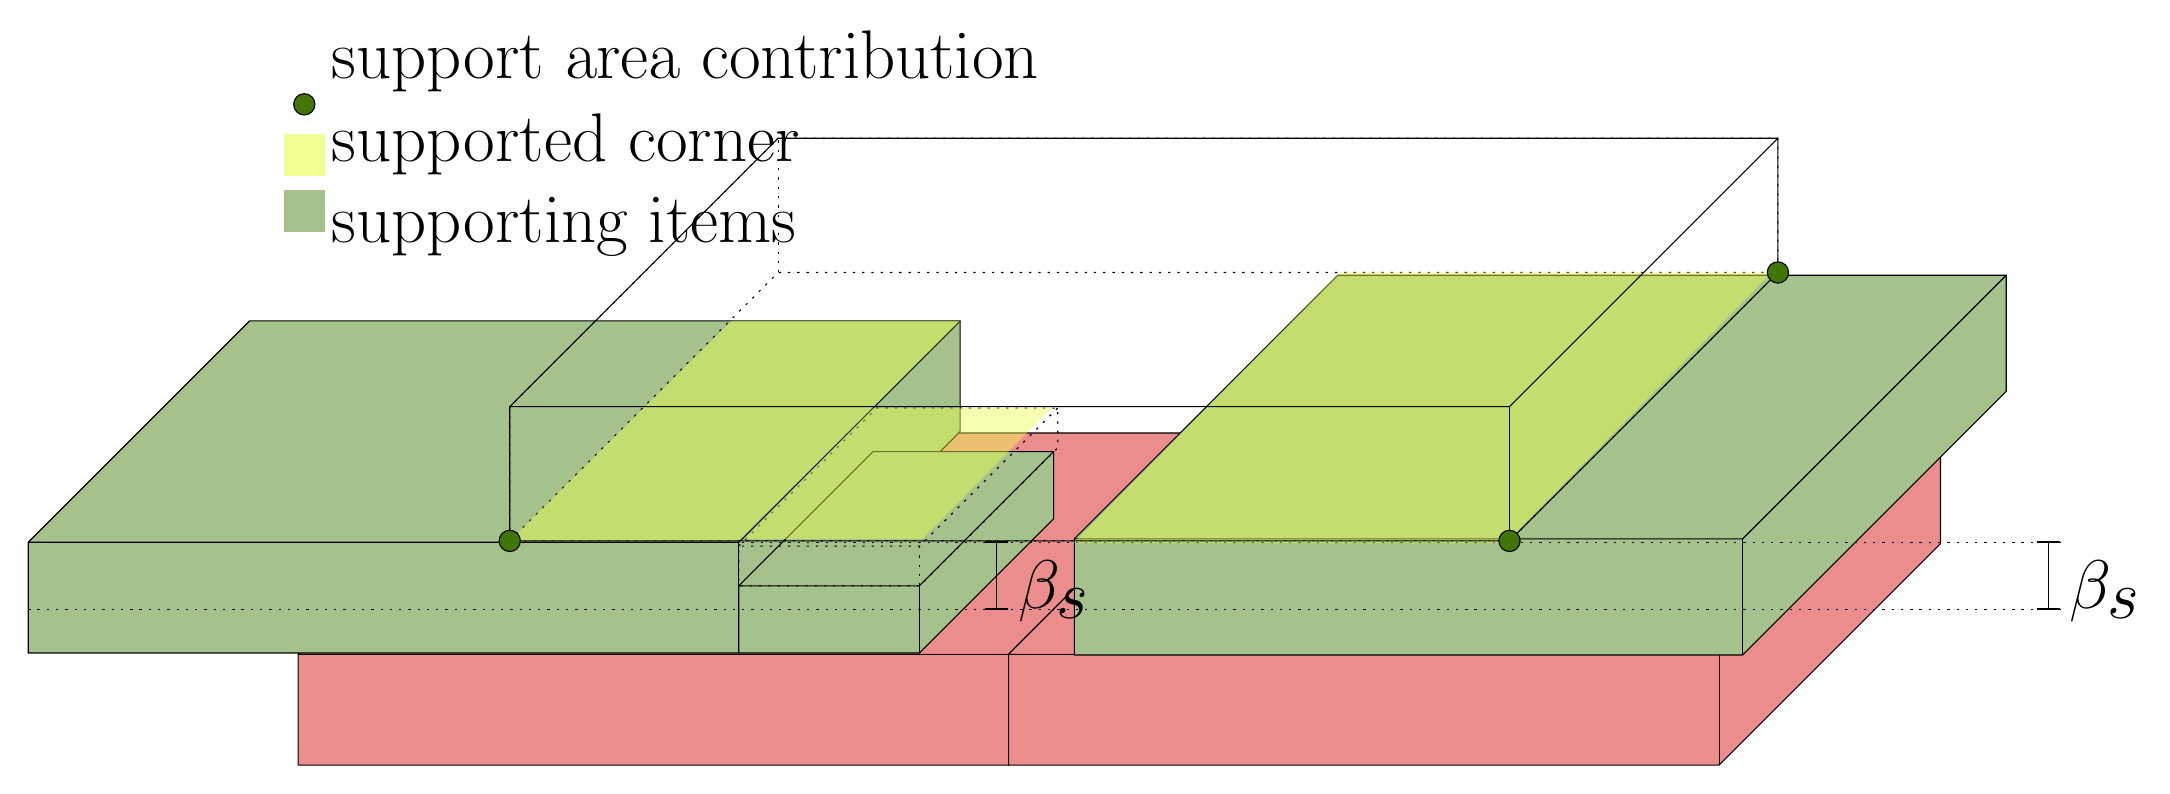
\begin{tikzpicture}[x=0.75pt,y=0.75pt,yscale=-1,xscale=1,font={\fontsize{50pt}{12}\selectfont}]
%uncomment if require: \path (0,479); %set diagram left start at 0, and has height of 479

%Shape: Cube [id:dp9411979483763162] 
\draw  [fill={rgb, 255:red, 236; green, 141; blue, 141 }  ,fill opacity=1 ] (194,306.67) -- (300.67,200) -- (643,200) -- (643,253.33) -- (536.33,360) -- (194,360) -- cycle ; \draw   (643,200) -- (536.33,306.67) -- (194,306.67) ; \draw   (536.33,306.67) -- (536.33,360) ;
%Shape: Cube [id:dp993645103603593] 
\draw  [fill={rgb, 255:red, 236; green, 141; blue, 141 }  ,fill opacity=1 ] (536.33,306.67) -- (643,200) -- (985.33,200) -- (985.33,253.33) -- (878.67,360) -- (536.33,360) -- cycle ; \draw   (985.33,200) -- (878.67,306.67) -- (536.33,306.67) ; \draw   (878.67,306.67) -- (878.67,360) ;
%Shape: Cube [id:dp23986673546182513] 
\draw  [fill={rgb, 255:red, 165; green, 194; blue, 140 }  ,fill opacity=1 ] (64,252.67) -- (170.67,146) -- (513,146) -- (513,199.33) -- (406.33,306) -- (64,306) -- cycle ; \draw   (513,146) -- (406.33,252.67) -- (64,252.67) ; \draw   (406.33,252.67) -- (406.33,306) ;
%Shape: Cube [id:dp5474008601617114] 
\draw  [fill={rgb, 255:red, 165; green, 194; blue, 140 }  ,fill opacity=1 ] (406.33,273.67) -- (471,209) -- (558,209) -- (558,241.33) -- (493.33,306) -- (406.33,306) -- cycle ; \draw   (558,209) -- (493.33,273.67) -- (406.33,273.67) ; \draw   (493.33,273.67) -- (493.33,306) ;
%Shape: Cube [id:dp7313777533771082] 
\draw  [fill={rgb, 255:red, 165; green, 194; blue, 140 }  ,fill opacity=1 ] (568,251) -- (695,124) -- (1017,124) -- (1017,180) -- (890,307) -- (568,307) -- cycle ; \draw   (1017,124) -- (890,251) -- (568,251) ; \draw   (890,251) -- (890,307) ;
%Shape: Cube [id:dp9978562503762016] 
\draw  [dash pattern={on 0.84pt off 2.51pt}] (907,122.67) -- (777.67,252) -- (296,252) -- (296,187.33) -- (425.33,58) -- (907,58) -- cycle ; \draw  [dash pattern={on 0.84pt off 2.51pt}] (296,252) -- (425.33,122.67) -- (907,122.67) ; \draw  [dash pattern={on 0.84pt off 2.51pt}] (425.33,122.67) -- (425.33,58) ;
%Shape: Cube [id:dp48964002783685845] 
\draw  [color={rgb, 255:red, 0; green, 0; blue, 0 }  ,draw opacity=1 ][fill={rgb, 255:red, 255; green, 255; blue, 255 }  ,fill opacity=0 ][dash pattern={on 0.84pt off 2.51pt}] (406.33,254.53) -- (472.86,188) -- (560,188) -- (560,207.14) -- (493.47,273.67) -- (406.33,273.67) -- cycle ; \draw  [color={rgb, 255:red, 0; green, 0; blue, 0 }  ,draw opacity=1 ][dash pattern={on 0.84pt off 2.51pt}] (560,188) -- (493.47,254.53) -- (406.33,254.53) ; \draw  [color={rgb, 255:red, 0; green, 0; blue, 0 }  ,draw opacity=1 ][dash pattern={on 0.84pt off 2.51pt}] (493.47,254.53) -- (493.47,273.67) ;
%Straight Lines [id:da26590658600836115] 
\draw    (1037.33,252.67) -- (1037.33,285) ;
\draw [shift={(1037.33,285)}, rotate = 270] [color={rgb, 255:red, 0; green, 0; blue, 0 }  ][line width=0.75]    (0,5.59) -- (0,-5.59)   ;
\draw [shift={(1037.33,252.67)}, rotate = 270] [color={rgb, 255:red, 0; green, 0; blue, 0 }  ][line width=0.75]    (0,5.59) -- (0,-5.59)   ;
%Straight Lines [id:da26590658600836116] 
\draw    (530.33,252.67) -- (530.33,285) ;
\draw [shift={(530.33,285)}, rotate = 270] [color={rgb, 255:red, 0; green, 0; blue, 0 }  ][line width=0.75]    (0,5.59) -- (0,-5.59)   ;
\draw [shift={(530.33,252.67)}, rotate = 270] [color={rgb, 255:red, 0; green, 0; blue, 0 }  ][line width=0.75]    (0,5.59) -- (0,-5.59)   ;
%Straight Lines [id:da8302030012021052] 
\draw  [dash pattern={on 0.84pt off 2.51pt}]  (64,285) -- (1044,285) ;
%Straight Lines [id:da5354149137938202] 
\draw  [dash pattern={on 0.84pt off 2.51pt}]  (64,252.67) -- (1044,252.67) ;
%Shape: Parallelogram [id:dp4597753988697182] 
\draw  [color={rgb, 255:red, 0; green, 0; blue, 0 }  ,draw opacity=0 ][fill={rgb, 255:red, 234; green, 255; blue, 77 }  ,fill opacity=0.45 ] (403,146) -- (513,146) -- (406,252) -- (296,252) -- cycle ;
%Shape: Parallelogram [id:dp9407100355043312] 
\draw  [color={rgb, 255:red, 0; green, 0; blue, 0 }  ,draw opacity=0 ][fill={rgb, 255:red, 234; green, 255; blue, 77 }  ,fill opacity=0.45 ] (471,188) -- (557,188) -- (494.86,251) -- (408.86,251) -- cycle ;
%Shape: Parallelogram [id:dp5499917231467685] 
\draw  [color={rgb, 255:red, 0; green, 0; blue, 0 }  ,draw opacity=0 ][fill={rgb, 255:red, 234; green, 255; blue, 77 }  ,fill opacity=0.45 ] (696,122.67) -- (904,122.67) -- (775.67,253) -- (567.67,253) -- cycle ;
%Shape: Cube [id:dp21506487392572304] 
\draw   (296,187.33) -- (425.33,58) -- (907,58) -- (907,122.67) -- (777.67,252) -- (296,252) -- cycle ; \draw   (907,58) -- (777.67,187.33) -- (296,187.33) ; \draw   (777.67,187.33) -- (777.67,252) ;
%Shape: Rectangle [id:dp8515603217170198] 
\draw  [color={rgb, 255:red, 0; green, 0; blue, 0 }  ,draw opacity=0 ][fill={rgb, 255:red, 234; green, 255; blue, 77 }  ,fill opacity=0.62 ] (187,56) -- (207,56) -- (207,76) -- (187,76) -- cycle ;
%Shape: Rectangle [id:dp8969674268045522] 
\draw  [color={rgb, 255:red, 0; green, 0; blue, 0 }  ,draw opacity=0 ][fill={rgb, 255:red, 165; green, 194; blue, 140 }  ,fill opacity=1 ] (187,83) -- (207,83) -- (207,103) -- (187,103) -- cycle ;
%Shape: Circle [id:dp08410160878408413] 
\draw  [fill={rgb, 255:red, 65; green, 117; blue, 5 }  ,fill opacity=1 ] (290.88,252) .. controls (290.88,249.17) and (293.17,246.88) .. (296,246.88) .. controls (298.83,246.88) and (301.13,249.17) .. (301.13,252) .. controls (301.13,254.83) and (298.83,257.13) .. (296,257.13) .. controls (293.17,257.13) and (290.88,254.83) .. (290.88,252) -- cycle ;
%Shape: Circle [id:dp20799682119759832] 
\draw  [fill={rgb, 255:red, 65; green, 117; blue, 5 }  ,fill opacity=1 ] (772.54,252) .. controls (772.54,249.17) and (774.84,246.88) .. (777.67,246.88) .. controls (780.5,246.88) and (782.79,249.17) .. (782.79,252) .. controls (782.79,254.83) and (780.5,257.13) .. (777.67,257.13) .. controls (774.84,257.13) and (772.54,254.83) .. (772.54,252) -- cycle ;
%Shape: Circle [id:dp9242580914559287] 
\draw  [fill={rgb, 255:red, 65; green, 117; blue, 5 }  ,fill opacity=1 ] (901.88,122.67) .. controls (901.88,119.84) and (904.17,117.54) .. (907,117.54) .. controls (909.83,117.54) and (912.13,119.84) .. (912.13,122.67) .. controls (912.13,125.5) and (909.83,127.79) .. (907,127.79) .. controls (904.17,127.79) and (901.88,125.5) .. (901.88,122.67) -- cycle ;
%Shape: Circle [id:dp40386474009325335] 
\draw  [fill={rgb, 255:red, 65; green, 117; blue, 5 }  ,fill opacity=1 ] (191.88,41.67) .. controls (191.88,38.84) and (194.17,36.54) .. (197,36.54) .. controls (199.83,36.54) and (202.13,38.84) .. (202.13,41.67) .. controls (202.13,44.5) and (199.83,46.79) .. (197,46.79) .. controls (194.17,46.79) and (191.88,44.5) .. (191.88,41.67) -- cycle ;

% Text Node
\draw (1046,260.07) node [anchor=north west][inner sep=0.75pt]    {$\beta_{s}$};
% Text Node
\draw (540,260.07) node [anchor=north west][inner sep=0.75pt]    {$\beta_{s}$};
% Text Node
\draw (209,5) node [anchor=north west][inner sep=0.75pt]   [align=left] {support area contribution};
% Text Node
\draw (209,85) node [anchor=north west][inner sep=0.75pt]   [align=left] {supporting items};
% Text Node
\draw (209,45) node [anchor=north west][inner sep=0.75pt]   [align=left] {supported corner};


\end{tikzpicture}

    }
    \caption{Representation of an item with conditions \ref{support:area_support} and \ref{support:vertex_support} of vertical support given $\alpha_s = 0.5, \beta_s$}
    \label{fig:support}
\end{figure}

We propose an heuristic that combines a constructive heuristic with a beam-search algorithm.
The constructive heuristic is designed to solve a single-bin bin packing problem with vertical support, while the beam-search expands the heuristic's solutions by exploring different sequences of item placements.

%-----------------------------------------------------------------------------
% CONCLUSION
%-----------------------------------------------------------------------------
\section{Conclusions}
In this thesis, we presented an heuristic for the Three-Dimensional Bin Packing Problem with Vertical Support.
We modified the two-dimensional Extreme Points algorithm of \citet{crainic2008extreme} to consider vertical support.
We then used this modified algorithm in a constructive heuristic which builds solutions to the single bin three-dimensional bin packing problem by filling planes, generated based on the previously inserted items.
Finally, we introduced a beam-search algorithm which evaluates different sequences of item placements by using our proposed constructive heuristic, and removes duplicate solutions at each iteration.

Our heuristic achieved an average gap of $5.37\%$ against the best solutions provided by other heuristics, however we were able to solve the same problem in a fraction of their computational time.
We consider this as a great result since it states that our algorithm is competitive also in the realm of 3D-BPP without support.
We generated a data set of problem instances based on real-world products from our case study, and we used them to evaluate our heuristic.
In most configurations, our solutions exceeded the target metric of $70\%$ cage ratio, with some configurations having a negligible execution time.

Further research could introduce new practical constraints considered in the literature like family groupings, load-bearing, and compatibilities between items.
Improvement heuristics could also be adapted to account for the support constraint like, for example, space defragmentation techniques introduced by \cite{ZHU2012452}.

\begin{figure}
    \centering
    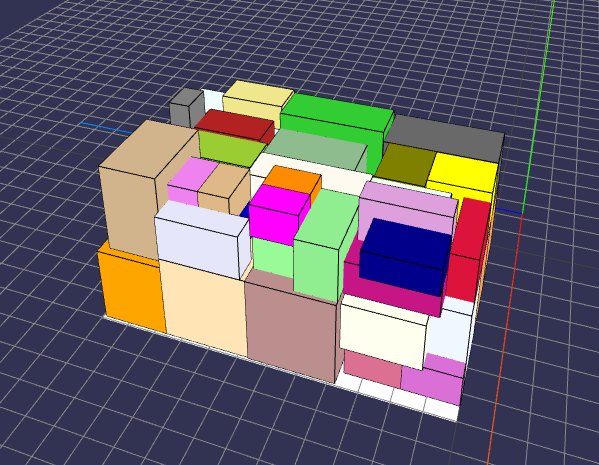
\includegraphics[width = \columnwidth]{tests/usecase/instance-82_k200.PNG}
    \caption{Solution to Instance 82 from case study tests}
\end{figure}

\begin{figure}
    \centering
    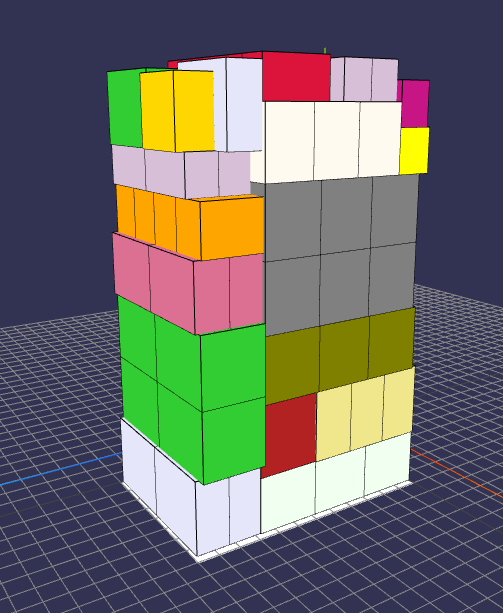
\includegraphics[width = \columnwidth]{tests/usecase/instance-66_bin1_k200.PNG}
    \caption{Solution to Instance 66, Bin 1 from case study tests}
\end{figure}

%---------------------------------------------------------------------------
%  ACKNOWLEDGEMENTS 
%---------------------------------------------------------------------------
\section{Acknowledgements}
My deepest gratitude goes to my supervisors, Prof. Ola Jabali and Dr. Davide Croci for their insights and support.
This work wouldn't have been possible without them.\\
\\
Many thanks to the team at ERMES-X s.r.l who provided me with the case study and the data used for our experiments.\\
\\
Many thanks to my family, my mom Patrizia, my father Severino, and my sister Giulia for always supporting me during this journey.
Last but not least, thanks to my colleagues Alberto, Edoardo, Mirko, and Kevin, that brightened every day at the university.

%---------------------------------------------------------------------------
%  BIBLIOGRAPHY
%---------------------------------------------------------------------------
% Remember to insert here only the essential bibliography of your work
\setcitestyle{numbers} % set the citation style to ``numbers''.
\bibliography{literature.bib} % automatically inserted and ordered with this command 

\end{document}